\begin{figure}
\centering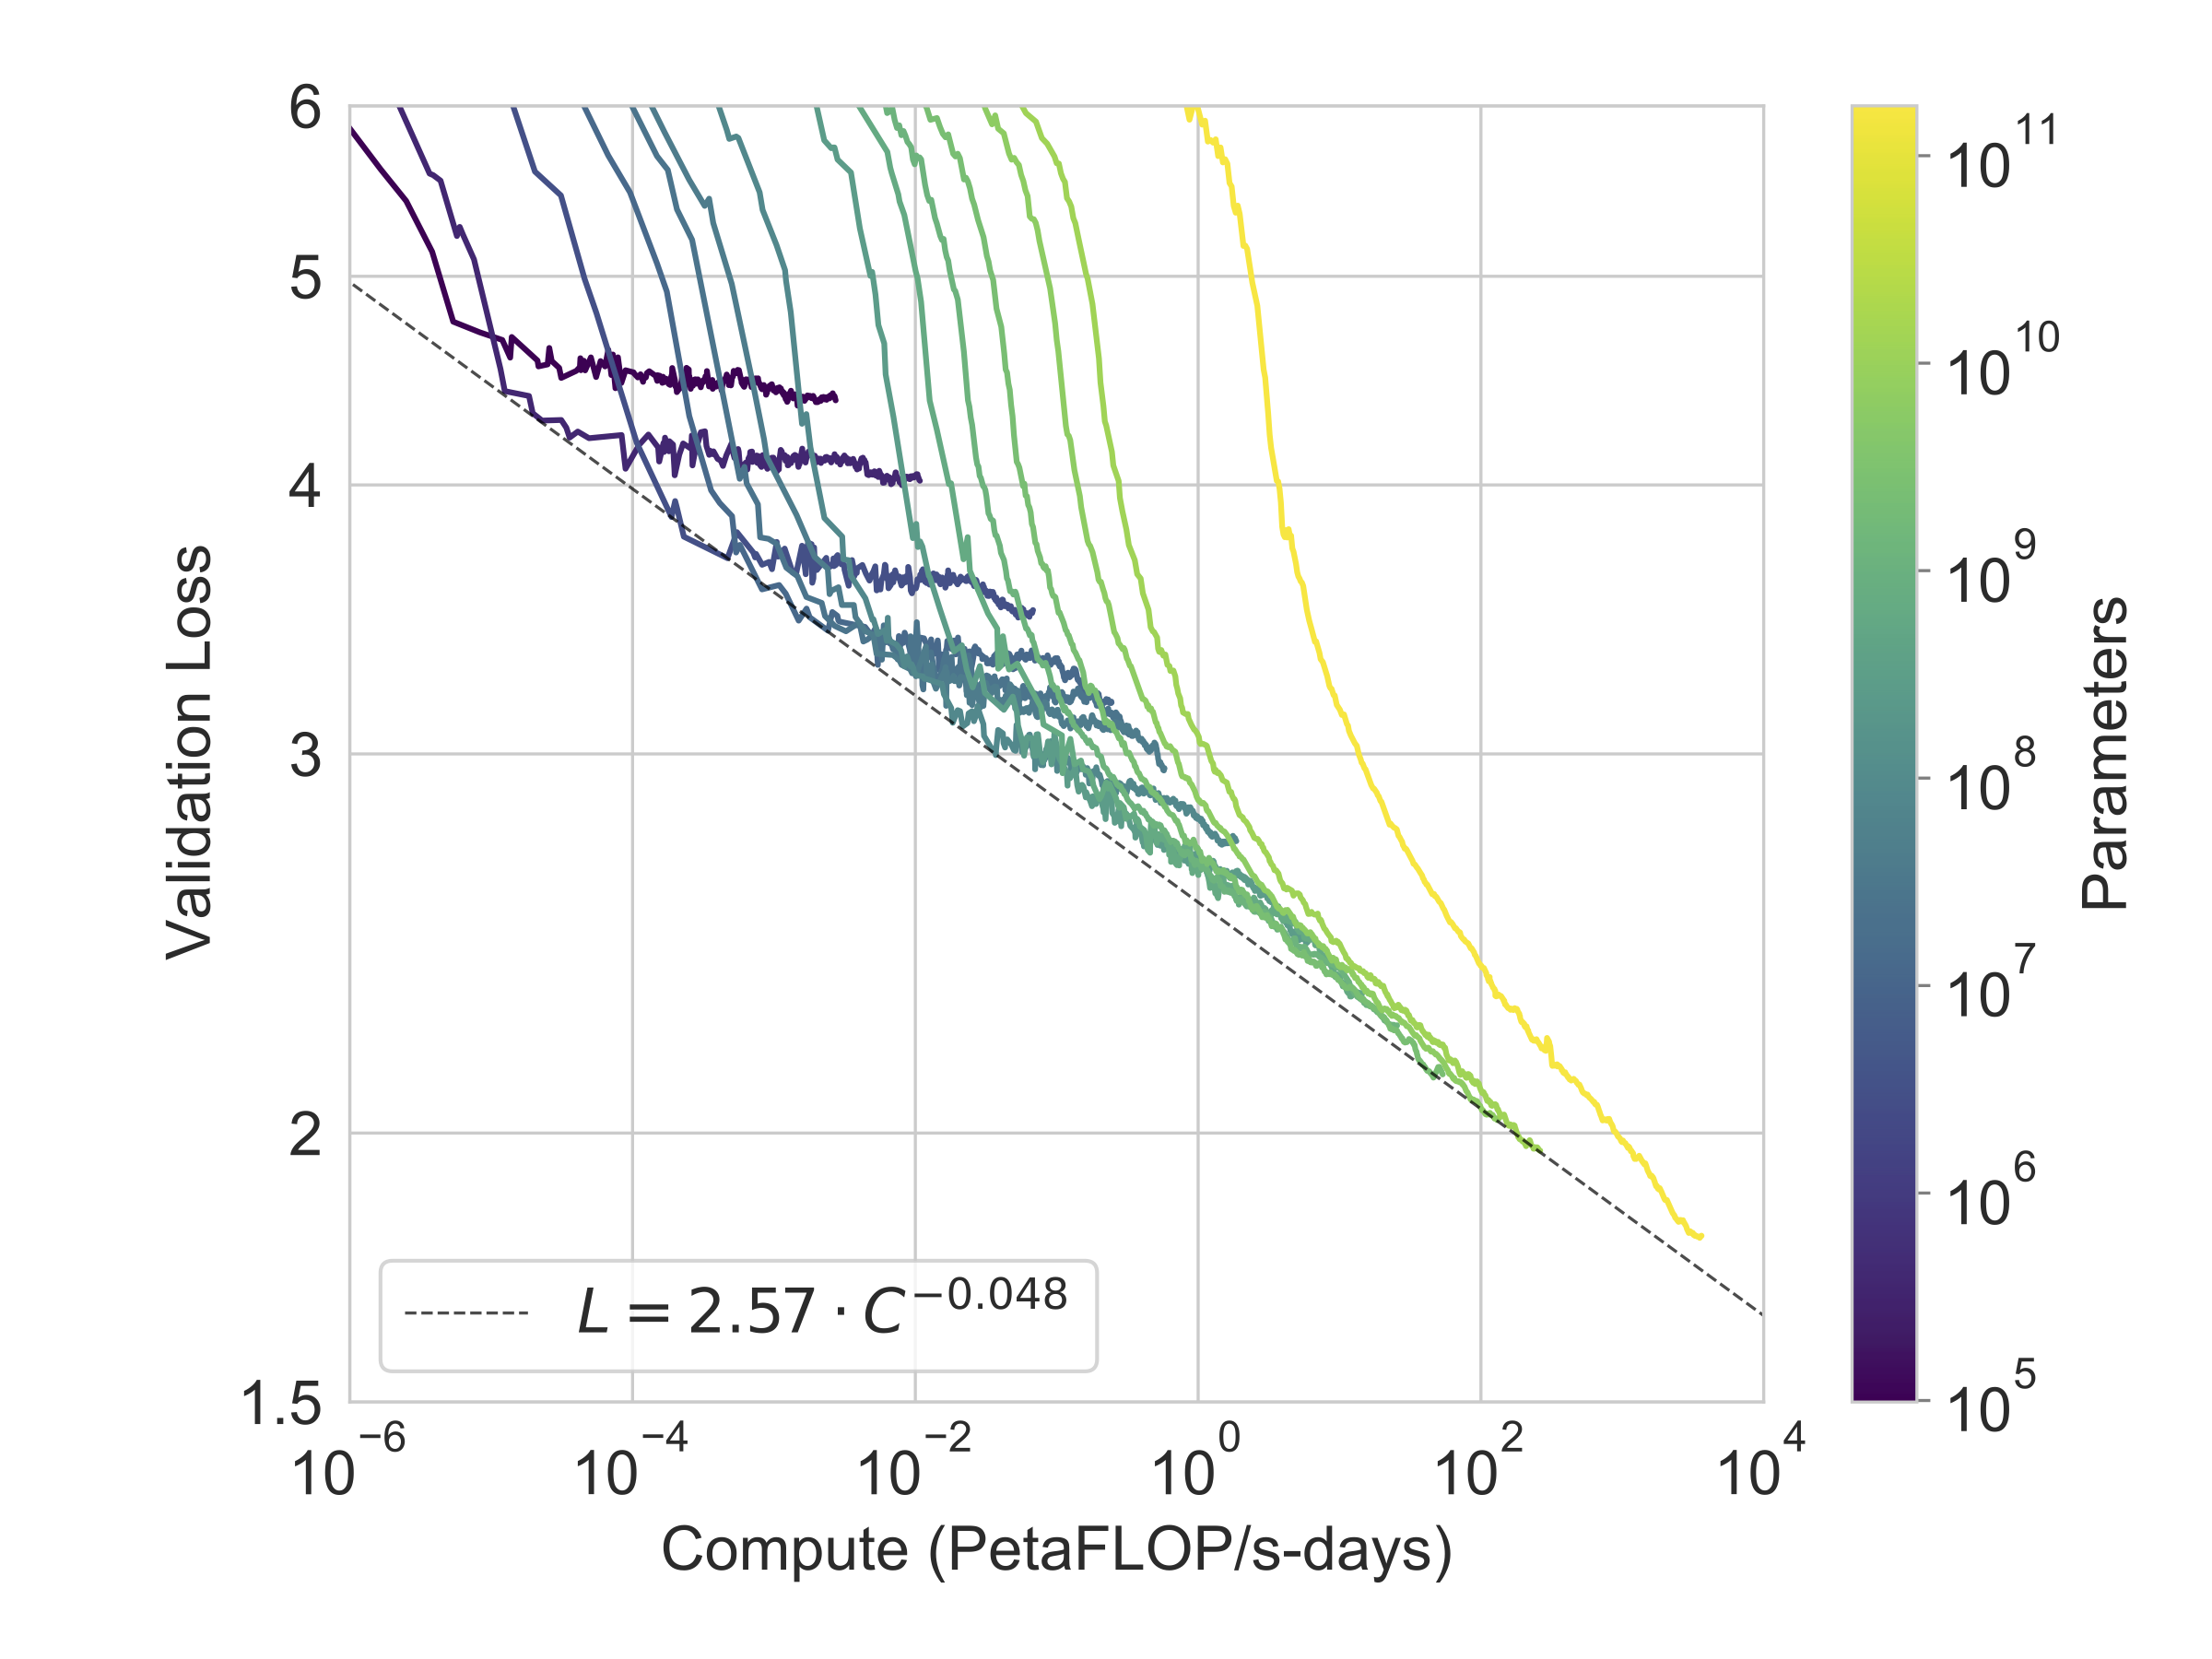
\includegraphics[width=0.7\linewidth]{graphs/img/LanguageModelingComputePareto.png}
\caption{\textbf{Smooth scaling of performance with compute.} Performance (measured in terms of cross-entropy validation loss) follows a power-law trend with the amount of compute used for training. The power-law behavior observed in \cite{kaplan2020scaling} continues for an additional two orders of magnitude with only small deviations from the predicted curve.  For this figure, we exclude embedding parameters from compute and parameter counts.}
\label{graph:compute}
\end{figure}

In Figure \ref{graph:compute} we display training curves for the 8 models described in Section \ref{section:Approach}. For this graph we also include 6 additional extra-small models with as few as 100,000 parameters. As observed in \cite{kaplan2020scaling}, language modeling performance follows a power-law when making efficient use of training compute. After extending this trend by two more orders of magnitude, we observe only a slight (if any) departure from the power-law. One might worry that these improvements in cross-entropy loss come only from modeling spurious details of our training corpus. However, we will see in the following sections that improvements in cross-entropy loss lead to consistent performance gains across a broad spectrum of natural language tasks.

Below, we evaluate the 8 models described in Section \ref{section:Approach} (the 175 billion parameter parameter GPT-3 and 7 smaller models) on a wide range of datasets. We group the datasets into 9 categories representing roughly similar tasks.  

In Section \ref{section:Language Modeling, Cloze, and Completion Tasks} we evaluate on traditional language modeling tasks and tasks that are similar to language modeling, such as Cloze tasks and sentence/paragraph completion tasks.  In Section \ref{section:Closed Book Question Answering / Knowledge Base Tasks} we evaluate on ``closed book'' question answering tasks: tasks which require using the information stored in the model’s parameters to answer general knowledge questions.  In Section \ref{section:Translation} we evaluate the model’s ability to translate between languages (especially one-shot and few-shot).  In Section \ref{section:Winograd-Style_Tasks} we evaluate the model’s performance on Winograd Schema-like tasks.  In Section \ref{section:Common_Sense_Reasoning} we evaluate on datasets that involve commonsense reasoning or question answering.  In Section \ref{section:Reading_Comprehension} we evaluate on reading comprehension tasks, in Section \ref{section:SuperGLUE} we evaluate on the SuperGLUE benchmark suite, and in \ref{section:ANLI} we briefly explore NLI.  Finally, in Section \ref{section:Synthetic_and_Qualitative_Tasks}, we invent some additional tasks designed especially to probe in-context learning abilities -- these tasks focus on on-the-fly reasoning, adaptation skills, or open-ended text synthesis. We evaluate all tasks in the few-shot, one-shot, and zero-shot settings.
